\section*{Theoretisch kader}
\subsection*{library in Android}
Voor de efficiënte implementatie van code door ontwikkelaars, zonder herhaaldelijk gebruik te maken van copy-paste, worden libraries gebruikt. Android-applicaties worden geprogrammeerd in Java of Kotlin, waarbij de build-tool Gradle wordt ingezet. Deze build-tool beheert de installatie van de benodigde libraries, zodat deze eenvoudig beschikbaar zijn voor integratie in de eigen code.
\newline
In tegenstelling tot een standaardapplicatie, die wordt gecompileerd naar een \gls{apk}, wordt een library gecompileerd naar een \gls{aar}. Deze \gls{aar}-bestanden kunnen vervolgens worden gepubliceerd naar publieke Gradle-plugins, waardoor ze eenvoudig herbruikbaar zijn in andere projecten.
\subsection*{lifecycle Android}
Ook belangrijk voor het maken van een library dat in de achtergrond locaties verzameld is rekening houden met de strenge regels van de android lifecycle.
\begin{figure}
    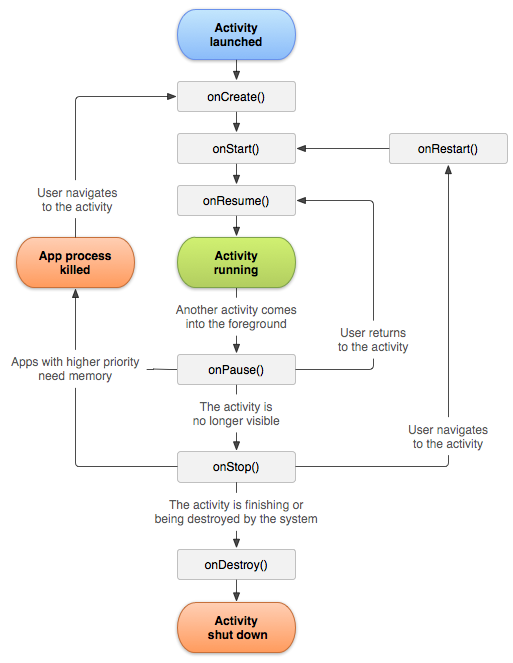
\includegraphics{images/activity_lifecycle.png}
    \label{fig:activity lifecycle}
\end{figure}
\subsection*{gps en telefoonmasten}
